\chapterbegin{Subrutinas y paso de parámetros}
\label{chp:Subrut}
\minitoc

{\bf Objetivos}: En esta sesión experimentaremos con las
subrutinas. Veremos en qué consiste la convención AAPCS y cómo
aplicarla tanto para llamar a funciones externas como para crear
nuestras propias funciones. Escribiremos un programa en C que llame
a funciones escritas en ensamblador. Por último explicaremos qué
son los registros de activación y cómo aplicarlos para almacenar
variables locales.

\section{Lectura previa}

\subsection{La pila y las instrucciones {\tt ldm} y {\tt stm}}

Se denomina pila de programa a aquella zona de memoria, organizada de
forma LIFO ({\it Last In, First Out}), que el programa emplea
principalmente para el almacenamiento temporal de datos.
%
Esta pila, definida en memoria, es fundamental para el funcionamiento
de las rutinas%
\footnote{
En este texto usaremos el término rutina (o subrutina) 
como la implementación
a bajo nivel de lo que en alto nivel se conoce como procedimientos
y funciones. La diferencia entre procedimiento y función, radica
en que las funciones proporcionan un valor de retorno. 
}%
, aspecto que se desarrollarán en esta
práctica.

El puntero de pila es {\tt r13} aunque por convención nunca se emplea esa
nomeclatura, sino que lo llamamos {\tt sp} ({\bf s}tack {\bf p}ointer o puntero
de pila). Dicho registro apunta siempre a la palabra de memoria que corresponde
a la cima de la pila (última palabra introducida en ella).

La pila tiene asociadas dos operaciones: {\tt push} (meter un elemento en la pila) y
{\tt pop} (sacar un elemento de la pila). En la operación {\tt push} primero
decrementamos en 4 (una palabra son 4 bytes) el registro {\tt sp} y luego escribimos
dicho elemento en memoria. Decimos que la pila crece hacia abajo.

\begin{lstlisting}[caption={Operación push},escapeinside={@}{@}]
        sub     sp, sp, #4
        str     r0, [sp]
\end{lstlisting}

Para sacar elementos de la pila tenemos la operación {\tt pop}, que primero extrae
el elemento de la pila y luego incrementa el puntero (decrece hacia arriba).

\begin{lstlisting}[caption={Operación pop},escapeinside={@}{@}]
        ldr     r0, [sp]
        add     sp, sp, #4
\end{lstlisting}

Para el procesador ARM estas instrucciones no existen. Sin embargo tenemos las
instrucciones {\tt stm} y {\tt ldm} que son mucho más potentes y el ensamblador
permite las pseudoinstrucciones {\tt push} y {\tt pop} que de forma transparente
traducirá a {\tt stm} y {\tt ldm}.

Un uso muy común de la pila es salvaguardar una serie de registros, que queremos
usar para hacer las operaciones que necesitemos pero que al final tenemos que
restaurar a sus valores originales. En un procesador típico escribiríamos algo así.

\begin{lstlisting}
        push    r1
        push    r2
        push    r4
        /* código que modifica los
           registros r1, r2 y r4   */
        pop     r4
        pop     r2
        pop     r1
\end{lstlisting}

Observa que el orden de recuperación de registros es inverso al de guardado. Pues
bien, en ARM lo tenemos mucho más fácil. Gracias a las instrucciones de carga/escritura
múltiple podemos meter los registros en una lista, empleando una única instrucción.

\begin{lstlisting}
        push    {r1, r2, r4}
        /* código que modifica los
           registros r1, r2 y r4   */
        pop     {r1, r2, r4}
\end{lstlisting}

En este caso el orden no es relevante, el procesador siempre usa el orden ascendente para
el {\tt push} y el descendente para el {\tt pop}, aunque nosotros por legibilidad siempre
escribiremos los registros en orden ascendente.

Las instrucciones {\tt ldm} y {\tt stm} tienen la siguiente sintaxis.

\begin{lstlisting}
    ldm{modo_direc}{cond} rn{!}, lista_reg
    stm{modo_direc}{cond} rn{!}, lista_reg
\end{lstlisting}

{\bf modo\_direc}
\begin{itemize}
  \item{\tt ia} Incrementa dirección después ({bf a}fter) de cada transferencia. Es el modo por defecto
                en caso de omitirlo.
  \item{\tt ib} Incrementa dirección antes ({bf b}efore) de cada transferencia.
  \item{\tt da} Decrementa después de cada transferencia.
  \item{\tt db} Decrementa antes de cada transferencia.
\end{itemize}

{\bf cond} Es opcional, son las mismas condiciones de los flags que vimos en el capítulo
          anterior, que permiten ejecutar o no dicha instrucción. En la práctica sólo las
          usamos para los saltos condicionales.

{\bf rn} Es el registro base, el cual apunta a la dirección inicial de memoria donde
          se hará la transferencia. El más común es {\tt sp} ({\tt r13}), pero puede
          emplearse cualquier otro.

{\bf !} Es un sufijo opcional. Si está presente, actualizamos {\tt rn} al final de la operación.

{\bf lista\_reg} Una lista de uno o más registros, que serán leídos o escritos en memoria. La
          lista va encerrada entre llaves y separada por comas. También podemos
          usar un rango de registros. En este ejemplo se almacenan los registros {\tt r3, r4,
          r5, r6, r10 y r12}.

\begin{lstlisting}
        stmdb   r1!, {r3-r6, r10, r12}
\end{lstlisting}

Si tenemos en cuenta que {\tt push} predecrementa, que {\tt pop} postincrementa y que ambas
actualizan el registro base (que sería {\tt sp}), la traducción de las pseudoinstrucciones
{\tt push \{r4, r6\}} y {\tt pop \{r4, r6\}} serían respectivamente.

\begin{lstlisting}
    stmdb sp!, {r4, r6}    /* push */
    ldmia sp!, {r4, r6}    /* pop  */
\end{lstlisting}

Nosotros sin embargo emplearemos los nemónicos {\tt push/pop}, mucho más fáciles de
recordar.

\subsection{Convención AAPCS}

Podemos seguir nuestras propias reglas, pero si queremos interactuar con las librerías
del sistema, tanto para llamar a funciones como para crear nuestras propias funciones
y que éstas sean invocadas desde un lenguaje de alto nivel, tenemos que seguir una serie
de pautas, lo que se denominamos AAPCS (Procedure Call Standard for the ARM Architecture).

\begin{enumerate}
  \item Podemos usar hasta cuatro registros (desde {\tt r0} hasta {\tt r3}) para pasar
        parámetros y hasta dos ({\tt r0} y {\tt r1}) para devolver el resultado.\newline
  \item No estamos obligados a usarlos todos, si por ejemplo la función sólo usa dos parámetros
        de tipo {\tt int} con {\tt r0} y {\tt r1} nos basta. Lo mismo pasa con el resultado,
        podemos no devolver nada (tipo {\tt void}), devolver sólo {\tt r0} (tipo {\tt int} ó un puntero
        a una estructura más compleja), o bien devolver {\tt r1:r0} cuando necesitemos enteros
        de 64 bits (tipo {\tt long long}).
  \item Los valores están alineados a 32 bits (tamaño de un registro), salvo en el caso de que
        algún parámetro sea más grande, en cuyo caso alinearemos a 64 bits. Un ejemplo de esto
        lo hemos visto en el Ejercicio 2.5, donde necesitábamos pasar dos parámetros: una cadena
        (puntero de 32 bits) y un entero tipo {\tt long long}. El puntero a cadena lo almacenábamos
        en {\tt r0} y el entero de 64 bits debe empezar en un registro par ({\tt r1} no vale)
        para que esté alineado a 64 bits, serían los registros {\tt r2} y {\tt r3}. En estos casos
        se emplea little endian, la parte menos significativa sería {\tt r2} y la de mayor peso, por
        tanto, {\tt r3}.
  \item El resto de parámetros se pasan por pila. En la pila se aplican las mismas reglas de
        alineamiento que en los registros. La unidad mínima son 32 bits, por ejemplo si queremos
        pasar un char por valor, extendemos de byte a word rellenando con ceros los 3 bytes
        más significativos. Lo mismo ocurre con los enteros de 64 bits, en el momento en que haya
        un sólo parámetro de este tipo, todos los demás se alinean a 64 bits.
  \item Es muy importante preservar el resto de registros (de {\tt r4} en
        adelante incluyendo {\tt lr}). La única excepción es el registro {\tt r12} que podemos
        cambiar a nuestro antojo. Normalmente se emplea la pila para almacenarlos al comienzo de
        la función y restaurarlos a la salida de ésta. Puedes usar como registros temporales
        (no necesitan ser preservados) los registros desde {\tt r0} hasta {\tt r3} que no se hayan
        empleado para pasar parámetros.
  \item La pila debe estar alineada a 8 bytes, esto quiere decir que de usarla para preservar
        registros, debemos reservar un número par de ellos. Si sólo necesitamos preservar un
        número impar de ellos, añadimos un registro más a la lista dentro del {\tt push},
        aunque no necesite ser preservado.
  \item Aparte de para pasar parámetros y preservar registros, también podemos usar la pila
        para almacenar variables locales, siempre y cuando cumplamos la regla de alinear a
        8 bytes y equilibremos la pila antes de salir de la función.
\end{enumerate}

Lo mejor para entender estas reglas es con una serie de ejemplos de menor a mayor complejidad
que veremos a lo largo de este capítulo.

\section{Ejemplos de aplicación}

\subsection{Funciones en ensamblador llamadas desde C}

En este primer ejemplo crearemos nuestras propias funciones generadoras de números
aleatorios, a las que llamaremos {\tt myrand} y {\tt mysrand}
(en sustitución a las {\tt rand} y {\tt srand} que ya existen en la librería).

\begin{lstlisting}[caption={Código del programa subrut1.c},label={lst:codigoPract3_1},escapeinside={@}{@}]
#include <stdio.h>

void main(void){
  int i;

  mysrand(42);
  for ( i= 0; i<5; i++ ){
    printf("%d\n", myrand());
  }
}
\end{lstlisting}

El programa principal lo hacemos en C, mientras que las funciones {\tt myrand} y {\tt mysrand}
las haremos en ensamblador. La implementación es sencilla, almacenamos la semilla en la variable
estática {\tt seed}, podemos cambiar el valor de la semilla en cualquier momento con la función
{\tt mysrand}, y recibir un número pseudoaleatorio de 15 bits con la función {\tt myrand}.
En realidad {\tt myrand} lo único que hace es aplicar una operación sencilla en la semilla
(multiplicación y suma) y extraer 15 bits de esta. El secreto del algoritmo reside en que se
han elegido unas constantes para la multiplicación y la suma de tal forma que la variable 
{\tt seed} pasará por todos los valores de 32 bits en una secuencia que a simple vista parece
aleatoria, pero que no lo es (por eso se llama pseudoaleatoria).

\begin{lstlisting}
short myrand(void){
  seed= seed*1103515245 + 12345;
  return seed>>16 & 0x7fff;
}

void mysrand(int x){
  seed= x;
}
\end{lstlisting}

Veamos en qué se traducen estas funciones en ensamblador.

\begin{lstlisting}[caption={Código del programa subrut1.s},label={lst:codigoPract3_2},escapeinside={@}{@}]
.data
seed:   .word   1
const1: .word   1103515245
const2: .word   12345

.text
.global myrand, mysrand
myrand: ldr     r1, =seed
        ldr     r0, [r1]
        ldr     r2, [r1, #4]
        mul     r3, r0, r2
        ldr     r0, [r1, #8]
        add     r0, r0, r3
        str     r0, [r1]
        mov     r0, r0, LSL #1
        mov     r0, r0, LSR #17
        bx      lr

mysrand:ldr     r1, =seed
        str     r0, [r1]
        bx      lr
\end{lstlisting}

Antes de nada ensamblamos, compilamos/enlazamos y ejecutamos estos archivos para
comprobar su correcto funcionamiento.

\begin{lstlisting}
pi@raspberrypi ~ $ as -o subrut1.o subrut1.s
pi@raspberrypi ~ $ gcc -o subrut1 subrut1.c subrut1.o
pi@raspberrypi ~ $ ./subrut1
2929
28487
11805
6548
9708
pi@raspberrypi ~ $
\end{lstlisting}

A diferencia de ejemplos anteriores, en nuestro código ensamblador no tenemos
ninguna función {\tt main} porque ésta la hemos implementado en C. Sin embargo
aparecen dos etiquetas después de la directiva {\tt .global}, que son
{\tt myrand} y {\tt mysrand}. Esto es fundamental si queremos que nuestras
funciones sean vistas desde el exterior, en este caso el programa en C.

Empecemos con la función más sencilla, {\tt mysrand}. Consta de 3 instrucciones.
En la primera de ellas apuntamos con {\tt r1} a la dirección donde se encuentra
la variable {\tt seed}. En la segunda pasamos el primer y único parámetro de la
función, {\tt r0}, a lo que apunta {\tt r1}, es decir, a la variable {\tt seed}.
Por último salimos de la función con la conocida instrucción {\tt bx lr}.

No hay más, no tenemos que devolver nada en {\tt r0} (la función devuelve el
tipo {\tt void}), ni tenemos que preservar registros, ni crear variables locales.

La otra función es un poco más compleja, aparte de requerir más cálculos debemos
devolver un valor. Aprovechamos que las 3 variables están juntas (en realidad las
dos últimas son constantes) para no tener que cargar 3 veces la dirección de cada
variable en un registro. Lo hacemos la primera vez con {\tt ldr r1, =seed}, y
accedemos a las variables con direccionamiento a registro con desplazamiento (
{\tt [r1], [r1, \#4] y [r1, \#8]}). Como no hay parámetros de entrada empleamos
los registros {\tt r0, r1, r2 y r3} como almacenamiento temporal, hacemos nuestros
cálculos, escribimos el resultado en la variable {\tt seed} y devolvemos el
resultado en el registro {\tt r0}.

\subsection{Funciones en ensamblador llamadas desde ensamblador}

Del ejemplo anterior pasamos a ensamblador la única parte que estaba escrita en
C, que era la función {\tt main}.

\begin{lstlisting}[caption={Código del programa subrut2.s},label={lst:codigoPract3_3},escapeinside={@}{@}]
.data
var1:   .asciz  "%d\n"
seed:   .word   1
const1: .word   1103515245
const2: .word   12345

.text
.global main
main:   push    {r4, r5}
        mov     r0, #42
        bl      mysrand
        mov     r4, #5
bucle:  bl      myrand
        mov     r1, r0
        ldr     r0, =var1
        bl      printf
        subs    r4, r4, #1
        bne     bucle
        pop     {r4, r5}
        bx      lr

myrand: ldr     r1, =seed
        ldr     r0, [r1]
        ldr     r2, [r1, #4]
        mul     r3, r0, r2
        ldr     r0, [r1, #8]
        add     r0, r0, r3
        str     r0, [r1]
        mov     r0, r0, LSL #1
        mov     r0, r0, LSR #17
        bx      lr

mysrand:ldr     r1, =seed
        str     r0, [r1]
        bx      lr
\end{lstlisting}

Como véis ya no hace falta poner a {\tt .global} las funciones {\tt myrand} y {\tt mysrand},
puesto que son de uso interno. Sin embargo sí lo hacemos con {\tt main}, ya que ahora sí
la implementamos en ensamblador. Al fin y al cabo {\tt main} es otra función más y por
tanto debe de seguir la normativa AAPCS.

Primero preservamos {\tt r4} y {\tt r5}. En realidad {\tt r5} no se modifica y no haría falta
preservarla, lo hacemos para alinear a 8 la pila. Luego llamamos a {\tt mysrand} con el valor 42
como primer y único parámetro. Inicializamos a 5 el contador del bucle, que almacenamos en
{\tt r4} y comenzamos el bucle. El bucle consiste en llamar a {\tt myrand} y pasar el resultado
devuelto de esta función al segundo parámetro de la función {\tt printf}, llamar a {\tt printf},
decrementar contador y repetir bucle hasta que el contador llegue a cero.

Una vez salimos del bucle recuperamos los registros {\tt r4} y {\tt r5} y devolvemos el control
al sistema {\tt bx lr}.

\subsection{Funciones recursivas}

El siguiente paso es implementar una función recursiva en ensamblador. Vamos a escoger la 
secuencia de Fibonacci por su sencillez, trataremos de imprimir los diez primeros números
de la secuencia. Se trata de una sucesión de números naturales en las que los dos primeros
elementos valen uno y los siguientes se calculan sumando los dos elementos anteriores.
Los diez primeros números serían los siguientes.

\begin{lstlisting}
1, 1, 2, 3, 5, 8, 13, 21, 34, 55...
\end{lstlisting}

Este es código en un lenguaje de alto nivel como C que imprime la anterior secuencia.

\begin{lstlisting}[caption={Código del programa subrut3.c},label={lst:codigoPract3_4},escapeinside={@}{@}]
#include <stdio.h>

int fibonacci(int n){
  if( n < 2 )
    return 1;
  else
    return fibonacci(n-1) + fibonacci(n-2);
}

void main(void){
  int i;

  for ( i= 0; i<10; i++ )
    printf("%d\n", fibonacci(i));
}
\end{lstlisting}

Lo que vamos a explicar ahora es cómo crear variables locales dentro de una función. Aunque en
C no necesitemos variables locales para la función fibonacci, sí nos hará falta en ensamblador,
en concreto dos variables: una para acumular la suma y otra para mantener el parámetro de entrada.

Para ello vamos a emplear la pila, que hasta ahora sólo la dedicábamos para salvaguardar los
registros mayores de {\tt r4} en la función. En realidad encima de esto teníamos los parámetros
pasados por pila por el llamador, pero nunca los hemos usado porque han sido pocos los parámetros y
nos han bastado los registros para ello. Recuerda que el número de parámetros pasados por registros
es de 4 (dos en caso de parámetros de 64 bits), siempre en los registros desde {\tt r0} hasta
{\tt r3}, a partir de aquí si hay más parámetros, éstos se pasan por pila.

Las variables locales se alojan debajo del área de salvaguarda de registros, para ello hay que
hacer espacio decrementando el puntero de pila una cierta cantidad de bytes, e incrementando esa
misma cantidad justo antes de salir de la función. En la figura \ref{fig:pila} vemos el uso de la pila
de una función genérica.

\begin{figure}[h]
  \centering
    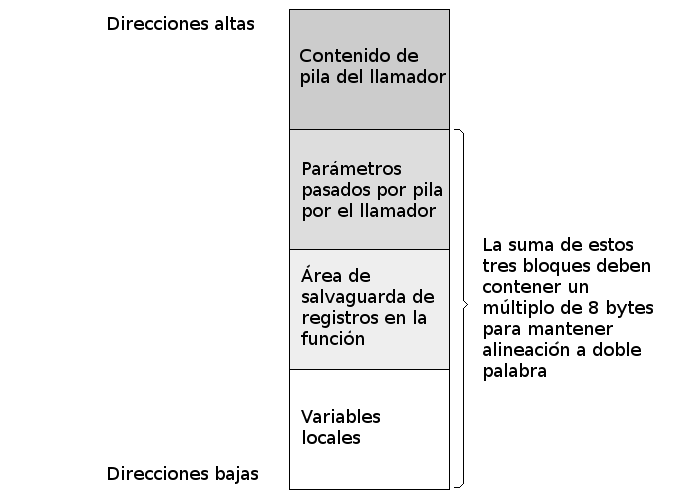
\includegraphics[width=14cm]{graphs/pila.png}
  \caption{Uso de la pila en una función}
  \label{fig:pila}
\end{figure}

Pues bien, en nuestro caso de la función fibonacci necesitamos 0 bytes para paso de parámetros,
4 bytes para salvaguarda de registros (sólo guardaremos {\tt lr}) y 8 bytes para nuestras
dos variables locales. Como la suma es de 12 bytes, que no es múltiplo de 8, redondeamos a 16
añadiendo una tercera variable local que no usaremos (también podríamos haber salvaguardado un
segundo registro).

Nuestro mapa particular lo podemos observar en la figura \ref{fig:pila2}.

\begin{figure}[h]
  \centering
    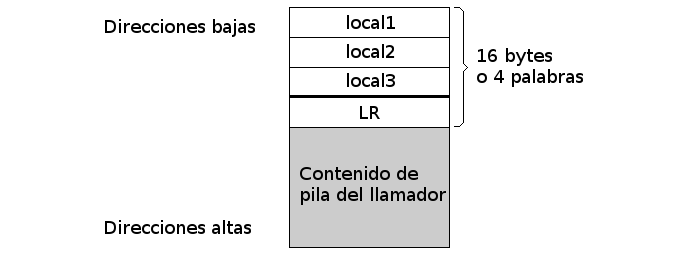
\includegraphics[width=14cm]{graphs/pila2.png}
  \caption{Uso de la pila en nuestra función}
  \label{fig:pila2}
\end{figure}

En teoría podemos encargarnos nosotros mismos de hacer toda la aritmética que conlleva el
uso de variables locales, pero en la práctica estamos más expuestos a cometer errores y
nuestro código es más ilegible. Las 3 variables locales ocupan 12 bytes, a la primera
accedemos con el direccionamiento {\tt [sp]} y a la segunda con {\tt [sp, \#4]} (la tercera
no la usamos). El código quedaría así.

\begin{lstlisting}
fibo:   push    {lr}
        sub     sp, #12
        cmp     r0, #2
        movlo   r0, #1
        blo     fib1
        sub     r0, #1
        str     r0, [sp]
        bl      fibo
        str     r0, [sp, #4]
        ldr     r0, [sp]
        sub     r0, #1
        bl      fibo
        ldr     r1, [sp, #4]
        add     r0, r1
fib1:   add     sp, #12
        pop     {lr}
        bx      lr
\end{lstlisting}

Siguiendo el orden de la pila, primero salvaguardamos {\tt lr} y luego hacemos espacio para
3 palabras con {\tt sub sp, \#12} en el comienzo de la función; al acabar restauramos en orden
inverso, primero restauramos los 12 bytes de las variables locales y luego recuperamos {\tt lr}.

Nuestra función tiene dos ramas, en una se comprueba que el parámetro sea menor de 2, y si lo
es devolvemos el valor 1 y salimos de la función. En la otra rama invocamos nuestra propia
función recursivamente dos veces, sumamos el resultado y devolvemos la suma al salir de la
función.

El truco para hacer el código más legible es nombrando las 3 variables locales y la longitud
mediante la directiva {\tt .equ} (también nos valdría su alias {\tt .set}). Partimos del valor
0 de desplazamiento en la primera variable local y vamos encadenando, a cada elemento le
corresponde la longitud más la posición del anterior. Así, si necesitamos modificar alguna
variable tan sólo tendremos en cuenta la anterior y la siguiente, no tenemos que modificar
toda la estructura.

\begin{lstlisting}
        .equ    local1,   0
        .equ    local2,   4+local1
        .equ    local3,   4+local2
        .equ    length,   4+local3
\end{lstlisting}

Con esta nueva filosofía el código queda menos críptico.

\begin{lstlisting}
fibo:   push    {lr}
        sub     sp, #length
        cmp     r0, #2
        movlo   r0, #1
        blo     fib1
        sub     r0, #1
        str     r0, [sp, #local1]
        bl      fibo
        str     r0, [sp, #local2]
        ldr     r0, [sp, #local1]
        sub     r0, #1
        bl      fibo
        ldr     r1, [sp, #local2]
        add     r0, r1
fib1:   add     sp, #length
        pop     {lr}
        bx      lr
\end{lstlisting}

Ya estamos en condiciones de mostrar el archivo completo.

\begin{lstlisting}[caption={Código del programa subrut3.s},label={lst:codigoPract3_5},escapeinside={@}{@}]
.data
var1:   .asciz  "%d\n"

.text
.global main
main:   push    {r4, lr}
        mov     r4, #0
bucle:  mov     r0, r4
        bl      fibo
        mov     r1, r0
        ldr     r0, =var1
        bl      printf
        add     r4, r4, #1
        cmp     r4, #10
        bne     bucle
        pop     {r4, lr}
        bx      lr

        .equ    local1,   0
        .equ    local2,   4+local1
        .equ    local3,   4+local2
        .equ    length,   4+local3

fibo:   push    {lr}
        sub     sp, #length
        cmp     r0, #2
        movlo   r0, #1
        blo     fib1
        sub     r0, #1
        str     r0, [sp, #local1]
        bl      fibo
        str     r0, [sp, #local2]
        ldr     r0, [sp, #local1]
        sub     r0, #1
        bl      fibo
        ldr     r1, [sp, #local2]
        add     r0, r1
fib1:   add     sp, #length
        pop     {lr}
        bx      lr
\end{lstlisting}

Lo único que nos faltaba era la función {\tt main}. La lista de {\tt .equ} puede
ir al comienzo, pero por claridad la ponemos justo antes de la función a la que
se va a aplicar. La función {\tt main} no tiene nada nuevo, lo único es que incrementamos
el contador {\tt r4} en lugar de decrementar porque lo necesitamos dicho valor como
parámetro para llamar a la función {\tt fibo}.

Para terminar con este ejemplo vamos a hacer una sencilla optimización. Observa un momento
la primera rama de la función. Si el parámetro es menor de dos tan sólo operamos con
un registro, {\tt r0}, tanto para comparar la entrada como para escribir el valor de retorno.
No se toca ningún registro más, no hemos modificado {\tt lr} porque no hemos llamado a ninguna
subrutina, tampoco hemos hecho uso de las variables locales.

La optimización consiste en procesar la primera rama antes de las operaciones con la pila,
de esta forma nos ahorramos algunos ciclos de reloj. Es un buen ejemplo para comprobar
lo flexibles que pueden ser las funciones: hay funciones en las que podemos evitar tratar
con la pila como en el listado \ref{lst:codigoPract3_3}, otras en las que no tenemos más
remedio, y un último caso en que podemos tener una mezcla de ambas.

\begin{lstlisting}[caption={Parte del código del programa subrut4.s},label={lst:codigoPract3_6},escapeinside={@}{@}]
fibo:   cmp     r0, #2
        movlo   r0, #1
        bxlo    lr
        push    {lr}
        sub     sp, #length
        sub     r0, #1
        str     r0, [sp, #local1]
        bl      fibo
        str     r0, [sp, #local2]
        ldr     r0, [sp, #local1]
        sub     r0, #1
        bl      fibo
        ldr     r1, [sp, #local2]
        add     r0, r1
        add     sp, #length
        pop     {lr}
        bx      lr
\end{lstlisting}

\subsection{Funciones con muchos parámetros de entrada}

Lo último que nos falta por ver es cómo acceder a los parámetros de una función por pila, para
lo cual necesitamos una función de al menos cinco parámetros. Lo más sencillo que se nos ocurre
es un algoritmo que evalue cualquier polinomio de grado 3 en el dominio de los enteros.


\begin{equation}
f(x) = ax^3 + bx^2 + cx + d
\label{eq:polinomio}
\end{equation}


Nuestra función tendría 5 entradas, una para cada coeficiente, más el valor de la $x$ que
sería el quinto parámetro que pasamos por pila.

Como siempre, comenzamos escribiendo el código en C.

\begin{lstlisting}[caption={Evaluador de polinomios subrut5.c},label={lst:codigoPract3_6},escapeinside={@}{@}]
int poly3(int a, int b, int c, int d, int x){
  return a*x*x*x + b*x*x + c*x + d;
}

void main(void){
  printf("%d\n%d\n%d\n",
          poly3(1, 2, 3, 4, 5), 
          poly3(1, -1, 1, -1, 8), 
          poly3(2, 0, 0, 0, 8));
}
\end{lstlisting}

Cuya salida es la siguiente.

\begin{lstlisting}
194
455
1024
\end{lstlisting}

El código completo es el siguiente.

\begin{lstlisting}[caption={Evaluador de polinomios subrut5.s},label={lst:codigoPract3_7},escapeinside={@}{@}]
.data
var1:   .asciz  "%d\n"

.text
.global main
main:   push    {r4, lr}
        mov     r0, #1
        mov     r1, #2
        mov     r2, #3
        mov     r3, #4
        mov     r4, #5
        push    {r4}
        bl      poly3
        add     sp, #4
        mov     r1, r0
        ldr     r0, =var1
        bl      printf

        mov     r0, #1
        mov     r1, #-1
        mov     r2, #1
        mov     r3, #-1
        mov     r4, #8
        push    {r4}
        bl      poly3
        add     sp, #4
        mov     r1, r0
        ldr     r0, =var1
        bl      printf

        mov     r0, #2
        mov     r1, #0
        mov     r2, #0
        mov     r3, #0
        mov     r4, #8
        push    {r4}
        bl      poly3
        add     sp, #4
        mov     r1, r0
        ldr     r0, =var1
        bl      printf
        pop     {r4, lr}
        bx      lr

        .equ    param5,   4*1  /* r4 */

poly3:  push    {r4}
        ldr     r4, [sp, #param5]
        smlabb  r3, r2, r4, r3
        smulbb  r2, r4, r4
        smlabb  r3, r1, r2, r3
        smulbb  r2, r2, r4
        smlabb  r0, r0, r2, r3
        pop     {r4}
        bx      lr
\end{lstlisting}

Vemos como hemos usado un {\tt .equ} para facilitar la legibilidad del código, así
accedemos al índice del quinto parámetro sin tener que hacer cálculos. El mapa de la
pila quedaría así.

\begin{figure}[h]
  \centering
    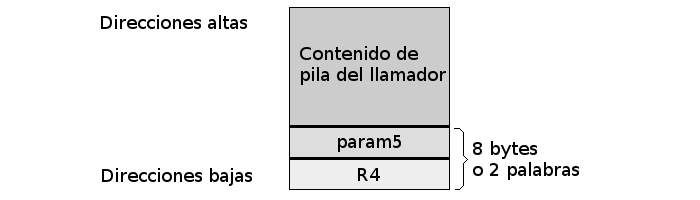
\includegraphics[width=14cm]{graphs/pila3.png}
  \caption{Mapa de pila de función poly3}
  \label{fig:pila3}
\end{figure}

Se pueden combinar los {\tt .equ} de variables locales con los de parámetros por pila,
por ejemplo si tuviésemos una función hipotética con 6 parámetros (dos de ellos pasados
por pila), 3 variables locales y salvaguarda de 3 registros, lo haríamos de la
siguiente forma.

\begin{lstlisting}
      .equ    local1,   0
      .equ    local2,   4+local1
      .equ    local3,   4+local2
      .equ    length,   4+local3
      .equ    param5,   4*3+length /* r4,r5,lr */
      .equ    param6,   4+param5*3

func: push    {r4, r5, lr}
      ...
\end{lstlisting}

Y éste sería el mapa de pila de nuestra hipotética función.

\begin{figure}[h]
  \centering
    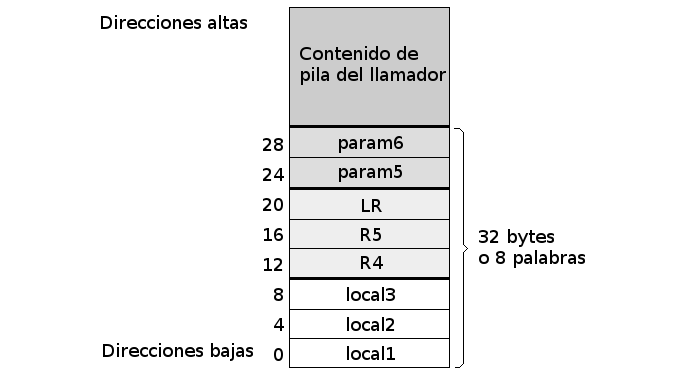
\includegraphics[width=14cm]{graphs/pila4.png}
  \caption{Mapa de función hipotética}
  \label{fig:pila4}
\end{figure}

Los números que hemos puesto números a la izquierda de cada elemento se
corresponden con las constantes que calcula el preprocesador para el
desplazamiento respecto al puntero de pila. De no haber empleado la lista
de {\tt .equ} tendríamos que calcular nosotros mismos estos desplazamientos,
y lo que es peor, el código perdería legibilidad. No es lo mismo poner
{\tt ldr r4, [sp, \#param5]}, que por ejemplo {\tt ldr r4, [sp, \#24]}, habría
que revisar a qué corresponde el desplazamiento {\tt \#24} o indicarlo como
comentario.

Por norma general en la arquitectura ARM se emplean muy poco las variables
locales, ya que operar con éstas implica guardarlas y restaurarlas de memoria,
para lo que se requieren instrucciones adicionales (recuerda que el procesador
no realiza operaciones aritméticas directamente en memoria). En lugar de
variables locales se suelen emplear directamente los registros que han sido
salvaguardados previamente con la instrucción {\tt push}, esto nos da juego
para trabajar con hasta 10 registros (desde {\tt r4} hasta {\tt r12},
incluyendo {\tt lr}) como almacén temporal para nuestras operaciones.

Veamos ahora nuestra función {\tt poly3}. Hemos salvaguardado {\tt r4} porque
necesitamos un almacén temporal donde operar con el quinto parámetro que
leeremos por pila. En esta función la pila está alineada a 8 bytes porque
usamos 4 bytes en el quinto parámetro más los 4 bytes de salvaguardar {\tt r4},
en total 8 bytes.

Todas los cálculos se condensan en 5 líneas donde se alternan las instrucciones
{\tt smlaxy} y {\tt smulxy}. Son instrucciones que multiplican/acumulan y
multiplican respectivamente números enteros. El comportamiento exacto de cada
instrucción viene detallado en el datasheet del procesador, aunque funciona
bastante bien buscándolas en google, suele aparecer la ayuda oficial en el primer
resultado de la búsqueda.

\begin{lstlisting}
  smlabb  r3, r2, r4, r3 /* r3= d+c*x             */
  smulbb  r2, r4, r4     /* r2= x^2               */
  smlabb  r3, r1, r2, r3 /* r3= d+c*x+b*x^2       */
  smulbb  r2, r2, r4     /* r2= x^3               */
  smlabb  r0, r0, r2, r3 /* r0= d+c*x+b*x^2+a*x^3 */
\end{lstlisting}

Como podéis observar, las instrucciones ARM son muy potentes, permiten
implementar en 5 instrucciones lo que en C nos habría costado 6
multiplicaciones y 4 sumas. Nótese como utilizamos como registros
intermedios {\tt r2, r3} los parámetros de entrada a medida que no los
necesitamos más.

Después de esto acaba la función con las habituales {\tt pop {r4}} y
{\tt bx lr}. Ya hemos terminado la función {\tt poly3}, ha quedado
bastante pequeña en tamaño. Todo lo contrario que la función {\tt main}.

La función {\tt main} es larga por varias razones: hacemos 3 llamadas
a {\tt poly3}, debemos introducir muchas constantes, algunas de ellas
en pila, y debemos imprimir los resultados y hacer el equilibrado de pila.

El equilibrado de pila consiste en incrementar {\tt sp} después de la
llamada a la función para desalojar los parámetros que previamente habíamos
introducido en la misma. Como en nuestro ejemplo pasamos por pila un
único parámetro de 4 bytes, lo que hacemos es incrementar {\tt sp} en 4 tras
cada llamada a {\tt poly3}.

Un detalle muy importante que no podemos observar en nuestro ejemplo, los
parámetros que pasamos por pila lo hacemos en orden inverso desde el último
al quinto. Esto es así porque la pila crece hacia abajo. Es más, es
aconsejable reusar los registros {\tt r0-r3} para introducir los
parámetros por pila. Si tuviésemos que pasar 6 parámetros, constantes del
1 al 6 lo haríamos así.

\begin{lstlisting}
        mov     r0, #6
        push    {r0}
        mov     r0, #5
        push    {r0}
        mov     r0, #1
        mov     r1, #2
        mov     r2, #3
        mov     r3, #4
\end{lstlisting}

Como véis no hay una forma clara y legible de introducir los parámetros
de una función. Tened cuidado con los push múltiples, no importa el orden
en que introduzcas los registros, el procesador siempre introduce en pila
el registro más alto y va hacia atrás hasta llegar al primero. Aprovechando
esto podemos mejorar el ejemplo anterior.

\begin{lstlisting}
        mov     r0, #5
        mov     r1, #6
        push    {r0, r1}
        mov     r0, #1
        mov     r1, #2
        mov     r2, #3
        mov     r3, #4
\end{lstlisting}

Por último vamos a mejorar un poco la velocidad de la función {\tt poly3} de
esta forma.

\begin{lstlisting}[caption={Parte de subrut6.s},label={lst:codigoPract3_8},escapeinside={@}{@}]
poly3:  sub     sp, #4
        ldr     r12, [sp, #param5]
        smlabb  r3, r2, r12, r3
        smulbb  r2, r12, r12
        smlabb  r3, r1, r2, r3
        smulbb  r2, r2, r12
        smlabb  r0, r0, r2, r3
        add     sp, #4
        bx      lr
\end{lstlisting}

¿En qué consiste la mejora? Pues que hemos usado el registro basura {\tt r12}, que
es el único que podemos emplear sin salvaguardarlo previamente en la lista del {\tt push}.
Esto nos quitaría el {\tt push} y el {\tt pop}, aunque en este ejemplo lo hemos
reemplazado por instrucciones {\tt sub} y {\tt add}. La razón es que debemos mantener
el puntero de pila en un múltiplo de 8. No obstante las instrucciones que no acceden
a memoria siempre son más rápidas que las que lo hacen, así que hemos ganado velocidad.

\subsection{Pasos detallados de llamadas a funciones}

Como ya hemos visto todos los casos posibles, hacemos un resumen de todo en una
serie de puntos desde que pasamos los parámetros en el llamador hasta que restauramos
la pila desde el llamador, pasando por la llamada a la función y la ejecución de la misma.

\begin{itemize}
  \item Usando los registros {\tt r0-r3} como almacén temporal, el llamador pasa por pila
        los parámetros quinto, sexto, etc... hasta el último. Cuidado con el orden,
        especialmente si se emplea un {\tt push} múltiple. Opcional, sólo si nuestra
        función tiene más de 4 parámetros.
  \item El llamador escribe los primeros 4 parámetros en {\tt r0-r3}. Opcional, nos
        podemos saltar este paso si nuestra función no tiene parámetros.
  \item El llamador invoca a la función con {\tt bl}. Este paso es obligatorio.
  \item Ya dentro de la función, lo primero que hace esta es salvaguardar los registros
        desde {\tt r4} que se empleen más adelante como registros temporales. También opcional.
  \item Decrementar la pila para hacer hueco a las variables locales. La suma de bytes
        entre paso de parámetros por pila, salvaguarda y variables locales debe ser
        múltiplo de 8, rellenar aquí hasta completar. Como este paso es opcional, en caso
        de no hacerlo aquí rellenar en el paso anterior.
  \item La función realiza las operaciones que necesite para completar su objetivo, accediendo
        a parámetros y variables locales mediante constantes {\tt .equ} para aportar mayor claridad
        al código. Se devuelve el valor resultado en {\tt r0} (ó en {\tt r1:r0} si es doble
        palabra).
  \item Incrementar la pila para revertir el alojamiento de variables locales.
  \item Recuperar con {\tt pop} la lista de registros salvaguardados.
  \item Retornar la función con {\tt bx lr} volviendo al código llamador, exactamente a la
        instrucción que hay tras el {\tt bl}. 
  \item El llamador equilibra la pila en caso de haber pasado parámetros por ella.
\end{itemize}

\section{Ejercicios}

\subsection{Mínimo de un vector}

Dado un vector de enteros y su longitud, escribe una función en ensamblador
que recorra todos los elementos del vector y nos devuelva el valor mínimo.
Para comprobar su funcionamiento, haz {\tt .global} la función y tras ensamblarla,
enlázala con este programa en C.

\begin{lstlisting}
#include <stdio.h>

int vect[]= {8, 10, -3, 4, -5, 50, 2, 3};

void main(void){
  printf("%d\n", minimo(vect, 8));
}
\end{lstlisting}

Hay muchas formas de calcular el mínimo de una lista de elementos, la más sencilla es
comparar todos los elemento con una variable, la cual actualizamos sólo si el elemento es
menor que la variable.

\begin{center}
\begin{myfbox}
\small
\begin{minipage}{0.92\linewidth}
\begin{center}
\begin{minipage}{0.6\linewidth}
\begin{verbatim}
  int minimo(int* v, int len){
    int i, min;

    min= v[0];
    for ( i= 1; i<len; i++ )
      if( v[i]<min )
        min= v[i];
    return min;
  }
\end{verbatim}
\end{minipage}
\end{center}
\begin{center}
\colorbox[gray]{1}{\rule{0cm}{7cm}\rule{11cm}{0cm}}
\end{center}
\end{minipage}
\end{myfbox}
\end{center}

\subsection{Media aritmética, macros y conteo de ciclos}

\subsubsection{Media aritmética}

Escribe una función en ensamblador que calcule la media aritmética (truncada porque
trabajamos con enteros) de dos números. Escribe también la función {\tt main} con 
cinco llamadas a {\tt media} con distintos parámetros.

\begin{center}
\begin{myfbox}
\small
\begin{minipage}{0.92\linewidth}
\begin{center}
\colorbox[gray]{1}{\rule{0cm}{4.5cm}\rule{11cm}{0cm}}
\end{center}
\end{minipage}
\end{myfbox}
\end{center}

Una vez hecho esto, supón que cada instrucción tarda un ciclo de reloj en ejecutarse.
Cuenta manualmente el número de ciclos que tarda la ejecución completa desde la primera
instrucción de {\tt main} hasta la última {\tt bx lr}, incluyendo ésta. En caso de una
llamada a subrutina cuenta todas las instrucciones que se ejecutan metiéndote en la
subrutina. La única excepción es {\tt bl printf}, que debes contar como un único ciclo.

Haz lo mismo pero usando la herramienta {\tt gdb} para comprobar el resultado anterior.
Recuerda no meterte dentro de los printf con {\tt ni}, en las llamadas a la función
{\tt abs} usa {\tt si}.

\subsubsection{Macros}

Hay una forma de acelerar las funciones, aunque sólo es práctica para funciones pequeñas
que se utilicen mucho. Se trata de escribir el contenido de la función en lugar de
llamar a la misma, y para evitar repetir siempre el mismo código utilizamos la directiva
{\tt .macro}. Con este truco nos ahorramos al menos la ejecución de las instrucciones
{\tt bl funcion} y {\tt bx lr}. El inconveniente es que el tamaño del ejecutable será
mayor.

Como ejemplo vamos a dar una implementación del método {\tt abs}.

\begin{lstlisting}[caption={Parte de subrut8.s},label={lst:codigoPract3_9},escapeinside={@}{@}]
      .macro  abs
        tst     r0, r0
        negmi   r0, r0
      .endm

.data
var1:   .asciz  "%d\n"

.text
.global main
main:   push    {r4, lr}
        mov     r0, #1
        bl      abs
        mov     r1, r0
        ldr     r0, =var1
        bl      printf

        mov     r0, #-2
        bl      abs
        mov     r1, r0
        ldr     r0, =var1
        bl      printf

        mov     r0, #3
        bl      abs
        mov     r1, r0
        ldr     r0, =var1
        bl      printf

        mov     r0, #-4
        bl      abs
        mov     r1, r0
        ldr     r0, =var1
        bl      printf
        pop     {r4, lr}
        bx      lr

abs:    tst     r0, r0
        negmi   r0, r0
        bx      lr
\end{lstlisting}

Borra el {\tt bl} antes del {\tt abs} para probar la versión con macros. Dentro de 
{\tt gdb} la secuencia de comandos para contar los pasos saltándose el
{\tt bl printf} junto con la cuenta es la siguiente.

\begin{lstlisting}
start / si 6 / ni / si 5 / ni /
/ si 5 / ni / si 5 / ni / si 2
6+1+(5+1)*3+2 = 27
\end{lstlisting}

Reescribe el ejercicio anterior de la media aritmética empleando macros en vez de
funciones.

\subsubsection{Conteo de ciclos}

Completa la siguiente tabla usando los dos tipos de conteo que acabamos de explicar.

\begin{center}
\small
\colorbox[gray]{0.9}{
%\arrayrulecolor{black}
\tabcolsep = 1mm
\begin{tabular}{ccccc}
&Ciclos contados & Ciclos contados & Ciclos manualmente & Ciclos, con {\tt gdb} \\
&manualmente & con {\tt gdb}       & empleando macros & y macros \\
media &
\colorbox[gray]{1}{\rule{0cm}{0.46cm}\rule{2.6cm}{0cm}} &
\colorbox[gray]{1}{\rule{0cm}{0.46cm}\rule{2.6cm}{0cm}} &
\colorbox[gray]{1}{\rule{0cm}{0.46cm}\rule{2.6cm}{0cm}} &
\colorbox[gray]{1}{\rule{0cm}{0.46cm}\rule{2.6cm}{0cm}} \\[1mm]
abs &
\colorbox[gray]{1}{\rule{0cm}{0.46cm}\rule{2.6cm}{0cm}} &
\colorbox[gray]{1}{\rule{0cm}{0.46cm}\rule{2.6cm}{0cm}} &
\colorbox[gray]{1}{\rule{0cm}{0.46cm}\rule{2.6cm}{0cm}} &
\colorbox[gray]{1}{\rule{0cm}{0.46cm}\rule{1.1cm}{0cm}27\rule{1.1cm}{0cm}} \\
\end{tabular}
\vspace{0.5ex}
}
\end{center}

Este conteo de ciclos es ilustrativo. En un procesador real sólo
las instrucciones simples tardan un ciclo de reloj, siempre y cuando
el resultado de la operación no se utilice en la instrucción posterior,
en cuyo la duración es de dos ciclos. Después hay instrucciones
complejas como las multiplicaciones, que necesitan 3 ciclos (más si hay
que añadir la penalización anterior). Por último están los casos 
más complejos. Por un lado tenemos los saltos condicionales, donde el
procesador hace una predicción de salto dentro de las 2 posibilidades
que hay, si se produce un fallo en la predicción se penalizan ciclos.
Por otro lado están los accesos a memoria, que tampoco tienen una
temporización constante porque está la caché por medio. Si se produce
un fallo de caché hay que añadir la penalización correspondiente.

\subsection{Algoritmo de ordenación}

Escoge un algoritmo de ordenación de entre los 4 siguientes.

\begin{itemize}
  \item Burbuja.
  \item Selección.
  \item Inserción.
  \item Quicksort.
\end{itemize}

E impleméntalo en ensamblador. Como ejemplo mostramos el código en C
del algoritmo de la burbuja.

\begin{lstlisting}[caption={Parte de subrut9.c},label={lst:codigoPract3_10},escapeinside={@}{@}]
#include <stdio.h>

int vect[]= {8, 10, -3, 4, -5, 50, 2, 3};

void ordena(int* v, int len){
  int i, j, aux;

  for ( i= 1; i<len; i++ )
    for ( j= 0; j<len-i; j++ )
      if( v[j] > v[j+1] )
        aux= v[j],
        v[j]= v[j+1],
        v[j+1]= aux;
}

void main(void){
  int i;

  ordena(vect, 8);
  for ( i= 0; i<8; i++ )
    printf("%d\n", vect[i]);
}
\end{lstlisting}

La lista de algoritmos está ordenada por dificultad, por lo que el algoritmo
{\tt Quicksort} es con diferencia el más difícil de implementar. Recomendamos
dejarlo para el final en caso de que el alumno decida realizar los 4 algoritmos
en ensamblador.

\chapterend{}
